% !TEX TS-program = pdflatex

%%%%%%%%%% NO MODIFICAR  %%%%%%
\documentclass[journal]{IEEEtran}
\IEEEoverridecommandlockouts
\usepackage{fancyhdr}
\usepackage{graphicx}
\usepackage[utf8]{inputenc}
\usepackage{color}
%\usepackage{hyperref}
\usepackage[hidelinks]{hyperref} 
\usepackage{wrapfig}
\usepackage{array}
\usepackage{multirow}
\usepackage{adjustbox}
\usepackage{nccmath}
\usepackage{subfigure}
\usepackage{amsfonts,latexsym} 
\usepackage{enumerate}
\usepackage{booktabs}
\usepackage{float}
\usepackage{threeparttable}
\usepackage{array,colortbl}
\usepackage{ifpdf}
\usepackage{rotating}
%\usepackage{cite}
\usepackage{stfloats}
\usepackage{url}
\usepackage{listings}
\usepackage[backend=biber]{biblatex} % Use biblatex with biber
\addbibresource{ref.bib}             % Reference your .bib file


%%%%%%%%%%%%%%%%%%%%%%%%%%%%%%%%%%%%%%%%%%%


\renewcommand\IEEEkeywordsname{Palabras clave}
%%%%%%%%%%%%%%%%%%%%%%%%%%%%%%%%%%%%%%%%%%%

% correct bad hyphenation here
\hyphenation{op-tical net-works semi-conduc-tor} 

\graphicspath{ {figs/} }  
\newcommand{\MYhead}{\smash{\scriptsize
\hfil\parbox[t][\height][t]{\textwidth}{\centering
\begin{picture}(-100,0) \put(-140,-20){
\includegraphics[width=40mm]{logoing}} \end{picture} \hspace{6.4cm}
COLORADO SCHOOL OF MINES\\ 
\hspace{2.8cm} GPGN 547A, PHYSICS, MECHANICS, AND PETROPHYSICS OF ROCKS TERM PAPER
}\hfil\hbox{}}}
\makeatletter
% normal pages
\def\ps@headings{%
\def\@oddhead{\MYhead}%
\def\@evenhead{\MYhead}}%
% title page
\def\ps@IEEEtitlepagestyle{%
\def\@oddhead{\MYhead}%
\def\@evenhead{\MYhead}}%
\makeatother
% make changes take effect
\pagestyle{headings}
% adjust as needed
\addtolength{\footskip}{0\baselineskip}
\addtolength{\textheight}{-1\baselineskip}

%%%%%%%%%%%%%%%%%%%%%%%%%%%%%%%%

\begin{document}

%Titulo
\title{\textcolor{black}{Permeability in Rock Physics: Foundations, Applications, and Advances in Reservoir Engineering}}      

%Datos
\author{Shenyao Jin\\shenyaojin@mines.edu} 

\maketitle

\begin{abstract}
    Permeability is a fundamental reservoir property that governs fluid flow through porous media and ultimately controls hydrocarbon recovery efficiency. This review systematically examines the role of permeability in reservoir engineering, from basic theoretical concepts to practical applications in enhanced oil recovery. We first establish the theoretical foundation of permeability-porosity relationships through the Kozeny-Carman model and related developments, demonstrating how pore structure and connectivity influence fluid flow capacity. The review then explores how permeability controls multiphase flow behavior through relative permeability and capillary pressure effects, which are critical for understanding fluid displacement processes. Applications in enhanced oil recovery are examined, with particular focus on how permeability heterogeneity affects water, polymer, and CO2 flooding performance. Special attention is given to the challenges posed by low-permeability formations such as tight reservoirs and shale, where traditional recovery mechanisms may be ineffective. Looking forward, we discuss emerging approaches in permeability characterization and prediction, including digital rock physics and machine learning techniques, which promise to improve our understanding and modeling of this crucial reservoir parameter.
\end{abstract}

\section{Introduction}

\subsection{Fundamentals of Permeability in Porous Media}

Permeability is a fundamental parameter governing fluid flow dynamics in reservoir rocks \parencite{corsano_low_1996}. The classical Darcy relationship is expressed as:

\begin{equation}
Q = -\frac{kA}{\mu} \left(\frac{\partial P}{\partial L}\right)
\end{equation}

\noindent where $Q$ represents volumetric flow rate, $k$ denotes intrinsic permeability, $A$ is the cross-sectional area perpendicular to flow, $\mu$ represents fluid viscosity, and $\partial P/\partial L$ describes the pressure gradient.

Unlike scalar properties such as porosity, permeability exhibits directional dependency, commonly displaying anisotropy between vertical and horizontal components. This can be expressed through a second-rank tensor:

\begin{equation}
\mathbf{k} = \begin{pmatrix}
k_{xx} & k_{xy} & k_{xz} \\
k_{yx} & k_{yy} & k_{yz} \\
k_{zx} & k_{zy} & k_{zz}
\end{pmatrix}
\end{equation}

The Kozeny-Carman equation provides a theoretical framework relating permeability to pore geometry:

\begin{equation}
k = \frac{\phi^3}{k_z S_p^2(1-\phi)^2}
\end{equation}

\noindent where $\phi$ represents porosity, $k_z$ is the Kozeny constant incorporating tortuosity effects, and $S_p$ denotes specific surface area \parencite{carman_fluid_1997}.

\begin{figure}[t]
    \centering
    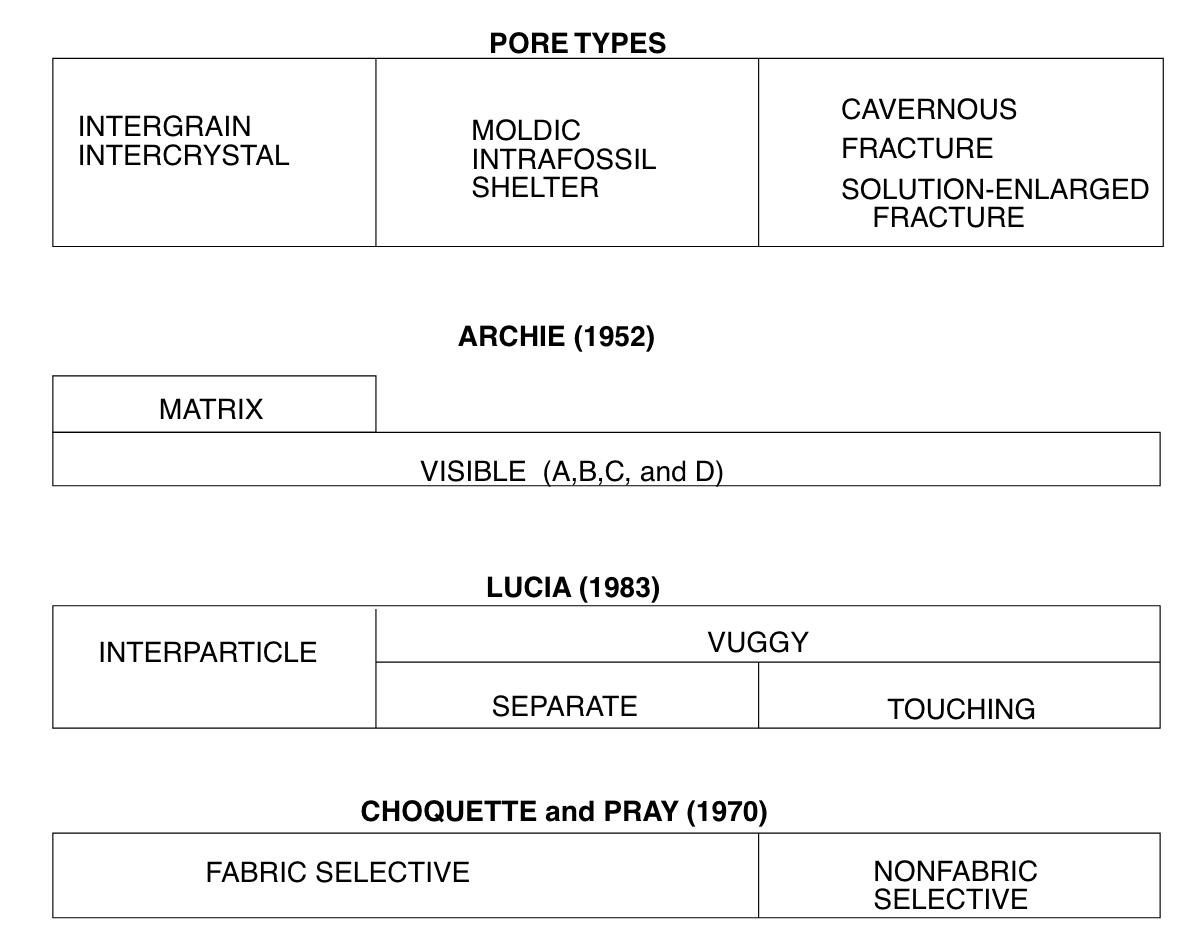
\includegraphics[width=0.9\linewidth]{fig2.png}
    \caption{Classification of carbonate pore types showing the relationships between different classification schemes. The progression from Archie's (1952) original classification through fabric-selectivity concepts (Choquette and Pray, 1970) to modern petrophysical classifications demonstrates the evolution in understanding how pore types influence permeability. Adapted from \textcite{f_jerry_lucia_2_rock-fabricpetrophysical_1995}.}
    \label{fig:pore_classification}
\end{figure}

The relationship between permeability and pore types is particularly important in carbonate rocks, where complex pore systems exist. Fig. \ref{fig:pore_classification} illustrates the classification of carbonate pore types, comparing different classification schemes and their relationships to permeability prediction. This classification framework is essential for understanding how different pore types contribute to overall reservoir permeability.

\subsection{Measurement and Characterization Methods}

Permeability measurement methods include laboratory core analysis and field-scale measurements, each with distinct advantages and limitations:

\begin{itemize}
    \item Laboratory core analysis using steady-state flow experiments requires careful control of pressure gradients, saturation history, and wettability equilibrium \parencite{chapuis_use_2003}.
    \item Field-scale well testing provides averaged permeability values over larger volumes, incorporating heterogeneity and natural fractures 1988\parencite{honarpour_relative-permeability_1988}.
\end{itemize}

The selection of appropriate measurement techniques and proper interpretation of results requires understanding how permeability measurements can be effectively applied to reservoir characterization and performance prediction.

\subsection{Applications in Reservoir Performance}

Modern approaches integrate rock fabric with petrophysical properties for improved reservoir characterization \parencite{f_jerry_lucia_2_rock-fabricpetrophysical_1995}. Three key petrophysical classes have been identified:

\begin{itemize}
    \item Class 1: Grainstones and large crystalline dolostones
    \item Class 2: Grain-dominated packstones and medium crystalline dolostones
    \item Class 3: Mud-dominated fabrics and fine crystalline dolostones
\end{itemize}

Recent developments include upscaling methods that calculate the full permeability tensor \parencite{schulz_beyond_2019}:

\begin{equation}
K_{ij} := \frac{1}{|Y|}\int_{Y_s}(\omega_j)_i dy
\end{equation}

where $Y_s$ represents the pore space and $\omega_j$ are solutions to supplementary cell problems.

The implementation of these advanced characterization methods has significant implications for:
\begin{itemize}
    \item Prediction of fluid flow patterns and reservoir performance
    \item Estimation of recovery factors and production rates
    \item Design of enhanced oil recovery operations
\end{itemize}

This integrated approach enables more reliable reservoir simulations and production forecasts by linking geological observations to engineering parameters, particularly in complex carbonate reservoirs where traditional porosity-permeability relationships may be insufficient.

While these theoretical frameworks provide the essential foundation for understanding permeability, translating theory into practice requires careful consideration of measurement approaches and their limitations. Moreover, the complexity of real reservoir systems necessitates an integrated understanding of how permeability interacts with other rock and fluid properties.

\section{Reservoir Quality and Permeability}

Having established the theoretical foundations and measurement approaches for permeability, we now examine how reservoir quality and various rock properties influence permeability in practice. This understanding is crucial for accurate prediction of fluid flow behavior in real reservoir systems.

\subsection{Basic Concepts and Relationships}
Reservoir quality is fundamentally controlled by the pore system characteristics and fluid flow capacity. While porosity quantifies storage capacity, permeability determines the ability of fluids to flow through the porous medium \parencite{yang_permeabilityporosity_2010}.
The Kozeny-Carman equation was developed to predict permeability based on measurable rock properties. Originally proposed by Kozeny and later modified by Carman, the equation relates permeability to porosity and specific surface area \parencite{chapuis_use_2003}:
\begin{equation}
k = \frac{c_0}{S_1^2}\frac{\phi^3}{(1-\phi)^2}
\end{equation}
\noindent where $k$ is permeability, $c_0$ is Kozeny's constant, $S_1$ is the specific surface per unit volume of solid matrix, and $\phi$ is porosity. The relationship was reformulated by Carman using:
\begin{equation}
S_1 = (1-\phi)S
\end{equation}
\noindent where $S$ represents the specific surface with respect to the unit volume of solid matrix. The Kozeny constant $c_0$ was empirically determined to be approximately $\frac{1}{5}$ for diverse geometries, accounting for tortuosity effects in real porous media \parencite{yang_permeabilityporosity_2010}.

\subsection{Controlling Factors on Permeability}

In real reservoir rocks, particularly in fine-grained sediments, permeability variations can span several orders of magnitude at a given porosity \parencite{yang_permeabilityporosity_2010}. Beyond the basic geometric factors captured in the Kozeny-Carman equation, this variation is controlled by:

\begin{figure}[t]
    \centering
    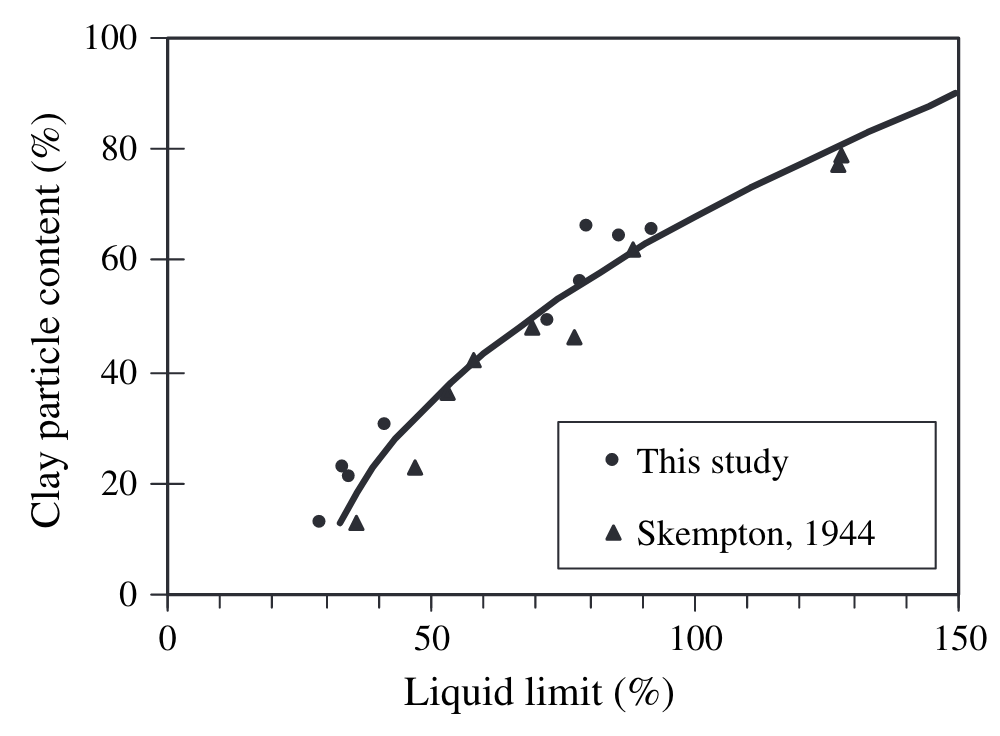
\includegraphics[width=0.8\linewidth]{fig1.png}
    \caption{Correlation between clay content and liquid limit for fine-grained clastic sediments. The strong relationship (based on 18 samples) enables estimation of clay content from liquid limit measurements, facilitating permeability prediction in mudstones. Adapted from \textcite{yang_permeabilityporosity_2010}.}
    \label{fig:clay_liquid}
\end{figure}
\begin{itemize}
    \item Clay content: The mass fraction of particles less than 2 microns in diameter serves as a key predictor of permeability variation. As shown in Fig. \ref{fig:clay_liquid}, clay content exhibits a strong correlation with liquid limit, providing a practical means to estimate clay content when direct measurements are unavailable. This relationship is particularly valuable for permeability prediction in fine-grained sediments.
    \item Pore geometry: Including aspects of pore size distribution and connectivity.
    \item Stress effects: The influence of effective stress on both porosity and permeability.
\end{itemize}
For mudstones, \textcite{yang_permeabilityporosity_2010} developed a more comprehensive relationship incorporating clay content (CF):
\begin{align}
\ln(K) = 69.59 - 26.79\cdot\text{CF} + 44.07\cdot\text{CF}^{0.5} + \nonumber\\
(53.61 - 80.03\cdot\text{CF} + 132.78\cdot\text{CF}^{0.5})\cdot e
\end{align}
\noindent where $K$ is permeability in m$^2$ and $e$ is the void ratio. This relationship reduces the predicted range of permeability from 2-5 orders of magnitude to one order at a given porosity.

The integration of these controlling factors with the fundamental equations provides a more complete framework for understanding reservoir quality and predicting flow behavior in heterogeneous reservoirs.

While understanding the relationship between reservoir quality and permeability provides crucial insights, these concepts must be extended to analyze actual fluid flow behavior in reservoir conditions. The presence of multiple fluid phases introduces additional complexity that must be carefully considered.

\section{Permeability and Fluid Flow}
Fluid flow through porous media is complex and cannot be described by theory alone. While absolute permeability represents the intrinsic flow capacity of a porous medium, the actual fluid transport in reservoirs typically involves multiple fluid phases, where the ability of each fluid to flow is reduced by the presence of other fluids.
The fundamental relationship governing single-phase fluid flow through porous media is Darcy's law, which relates the macroscopic velocity (flux) of a fluid to the pressure gradient through the permeability coefficient:
\begin{equation}
u + \frac{1}{\mu} K\nabla p = f
\end{equation}
where $u$ is the Darcy velocity, $\mu$ is fluid viscosity, $K$ is permeability tensor, $p$ is pressure, and $f$ represents external forces.
In multiphase flow systems, the relationship between capillary pressure ($P_c$), interfacial tension ($\sigma$), and pore radius ($r$) is described by:
\begin{equation}
P_c = P_{nw} - P_w = \frac{2\sigma\cos\theta}{r}
\end{equation}
where $P_{nw}$ and $P_w$ are the pressures in the non-wetting and wetting phases respectively, and $\theta$ is the contact angle \parencite{honarpour_relative-permeability_1988}. This relationship fundamentally controls fluid distribution at the pore scale.
For two-phase flow, relative permeability ($k_r$) relationships can be approximated using the Brooks-Corey model:
\begin{equation}
k_{rw} = k_{rw}^o(\frac{S_w - S_{wc}}{1 - S_{wc}})^{n_w}
\end{equation}
\begin{equation}
k_{rnw} = k_{rnw}^o(1 - \frac{S_w - S_{wc}}{1 - S_{wc}})^{n_{nw}}
\end{equation}

\begin{figure}[t]
    \centering
    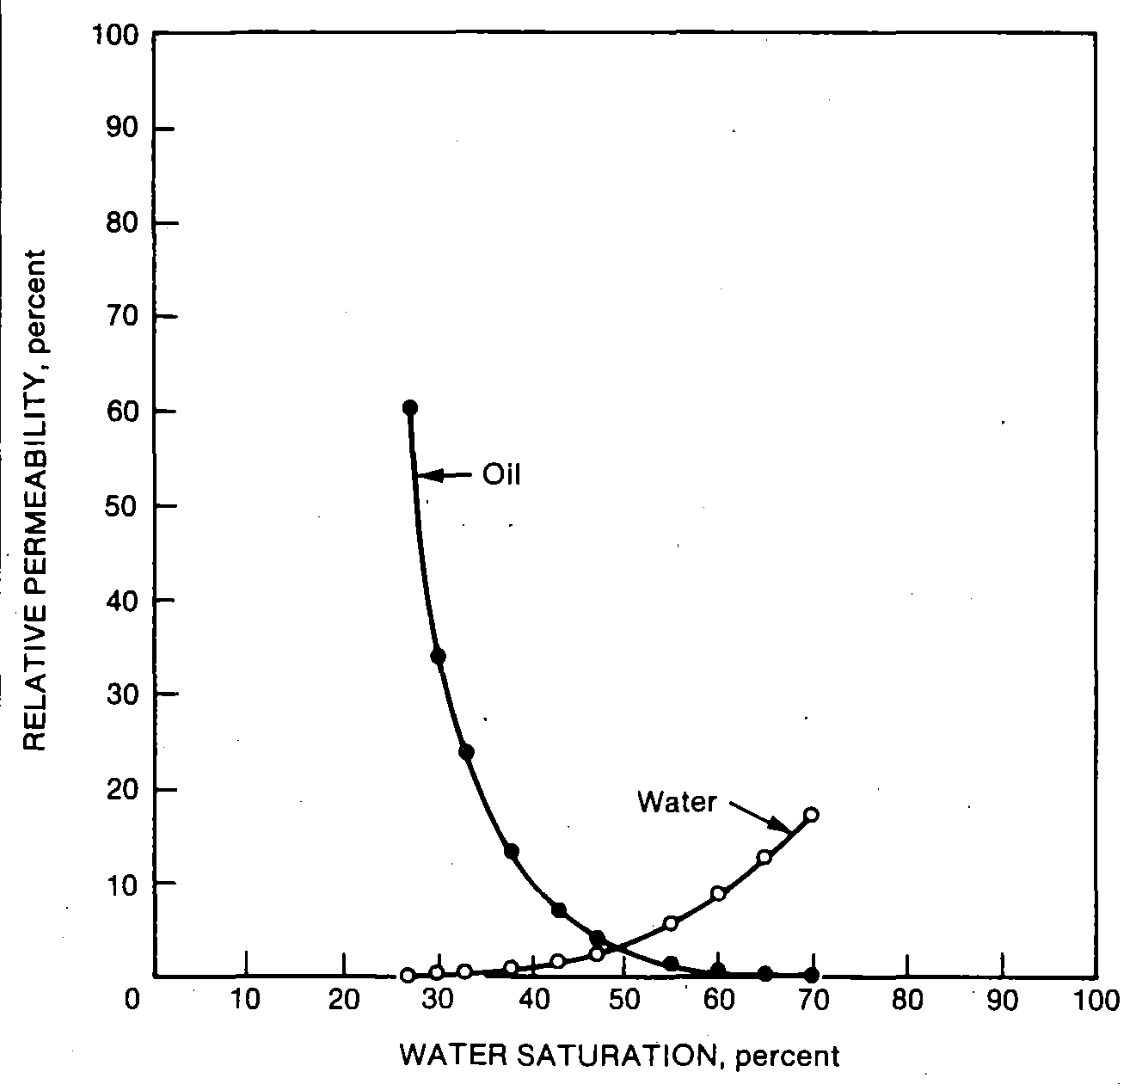
\includegraphics[width=0.8\linewidth]{fig4.png}
    \caption{Typical water/oil relative permeability curves showing the relationship between phase saturation and relative permeability. The crossover point and endpoints provide crucial information about reservoir wettability and multiphase flow characteristics. Note that water relative permeability increases while oil relative permeability decreases as water saturation increases. Adapted from \textcite{honarpour_relative-permeability_1988}.}
    \label{fig:rel_perm}
\end{figure}

where $S_w$ is water saturation, $S_{wc}$ is connate water saturation, and $n_w$ and $n_{nw}$ are empirical exponents for wetting and non-wetting phases respectively. Fig. \ref{fig:rel_perm} illustrates typical relative permeability curves for a water-oil system, demonstrating how the ability of each phase to flow varies with water saturation. These curves are fundamental to understanding multiphase flow behavior in reservoir rocks and are essential inputs for reservoir simulation and production forecasting.

The displacement efficiency in a reservoir is controlled by the competition between viscous and capillary forces, expressed through the capillary number:
\begin{equation}
N_c = \frac{v\mu}{\sigma}
\end{equation}
where $v$ is the characteristic velocity. This dimensionless number helps predict the dominant forces controlling fluid displacement.

As explained by \textcite{honarpour_relative-permeability_1988}, the sum of effective permeabilities for all phases is less than the absolute permeability due to interference between fluids sharing the same flow channels. The ratio of effective permeability to absolute permeability (relative permeability) has a first-order dependency on saturation level.

Two key experimental approaches are used to determine relative permeability: steady-state methods where multiple fluids are injected simultaneously until equilibrium is reached, and unsteady-state techniques where one fluid displaces another. Steady-state methods provide more reliable data but are time-consuming.

For carbonate rocks, \textcite{f_jerry_lucia_2_rock-fabricpetrophysical_1995} demonstrates that both relative permeability and capillary pressure characteristics are strongly influenced by pore geometry and wettability. The interplay between absolute permeability, relative permeability, and capillary pressure ultimately controls fluid displacement processes and recovery efficiency. \textcite{yang_permeabilityporosity_2010} show these relationships are heavily dependent on rock properties like clay content and pore size distribution.

The direction-dependent nature of permeability, particularly in layered sedimentary rocks, adds further complexity. This directional variation must be considered when predicting fluid flow patterns at both core and reservoir scales. While absolute permeability provides a starting point for understanding fluid flow capacity, reliable experimental data combined with appropriate flow models are essential for predicting reservoir performance.

The fundamental understanding of fluid flow behavior through permeable media directly impacts the effectiveness of enhanced oil recovery operations. The following section examines how permeability influences EOR processes and addresses the particular challenges posed by low permeability formations.

%%%%%%%%%%%%%%%%%%%%%%%%%%%%%%%

\section{Permeability in Enhanced Oil Recovery (EOR)}
Permeability plays a critical role in enhanced oil recovery (EOR) as it directly impacts fluid flow and ultimate recovery. This chapter examines the impact of miscible flooding on permeability and the challenges posed by low permeability reservoirs in EOR operations.

\subsection{Impact of Miscible Flooding on Permeability}
Miscible flooding can significantly alter reservoir permeability by affecting wettability and relative permeability relationships. Key findings from laboratory studies include:

\textbf{Wettability Effects:} Miscible flooding alters in-situ wettability in water-wet, intermediate-wet, and oil-wet systems, primarily through changes in endpoint oil and water permeabilities and saturation shifts in carbonates \parencite{rao_impact_1992}.

\begin{figure}[t]
    \centering
    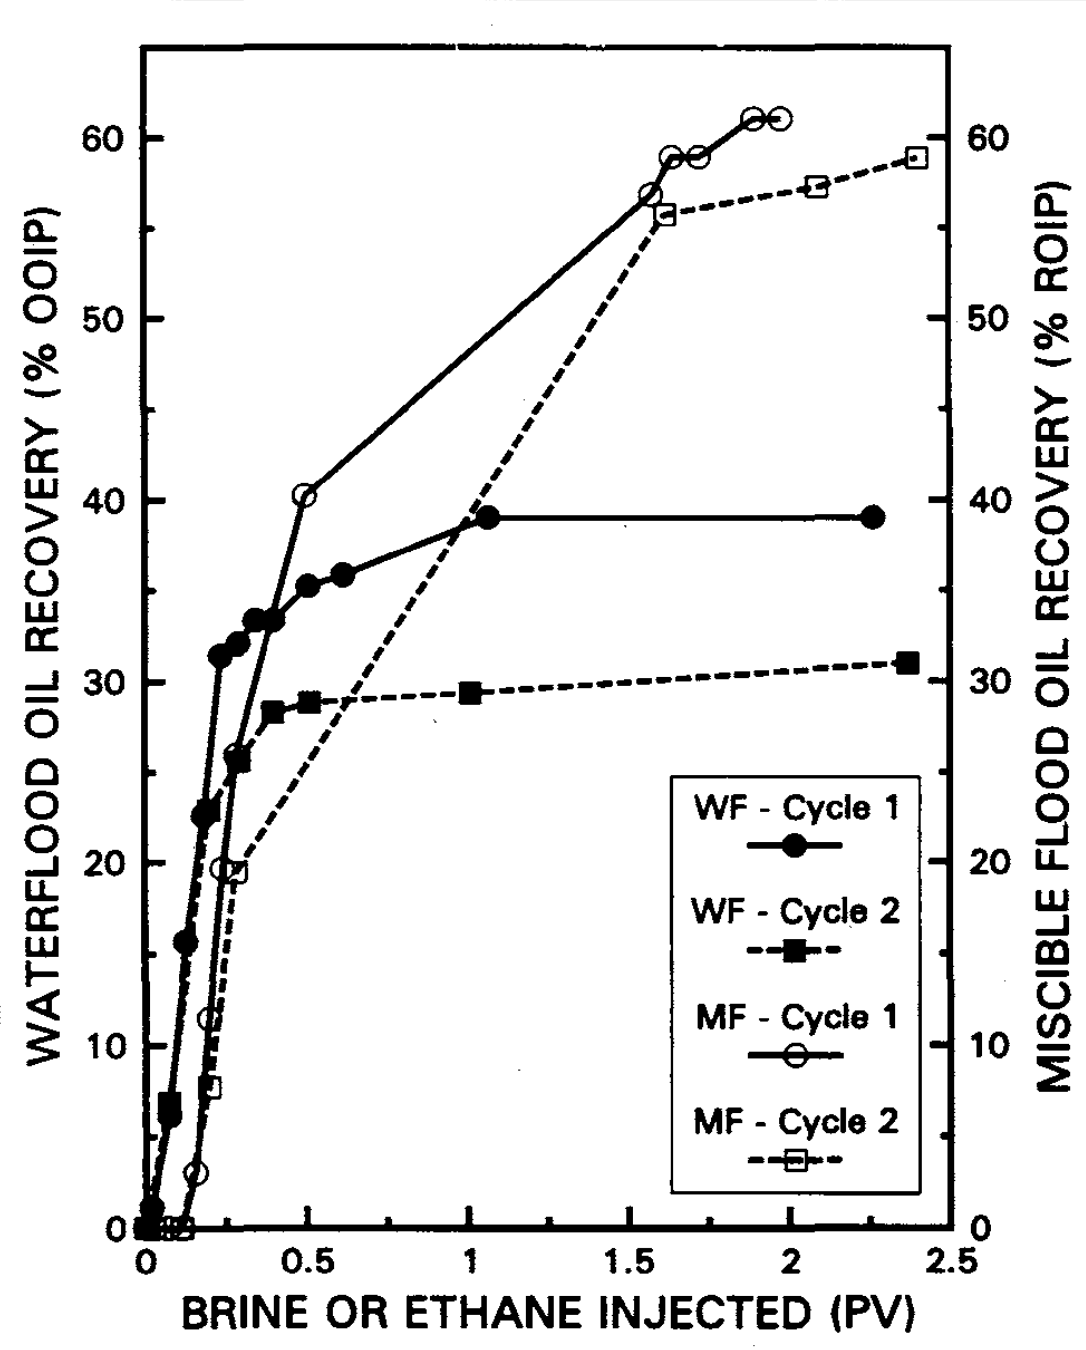
\includegraphics[width=0.8\linewidth]{fig3.png}
    \caption{Oil recovery performance during waterflood (WF) and miscible flood (MF) cycles in a water-wet reservoir system. The similar recovery profiles between cycles in water-wet conditions demonstrate the minimal impact of wettability alteration in such systems. MF = miscible flood and WF = waterflood. Adapted from \textcite{rao_impact_1992}.}
    \label{fig:miscible_recovery}
    \end{figure}

\textbf{Impact on Oil Recovery:} The influence of wettability alterations on oil recovery depends on initial wettability, as demonstrated in Fig. \ref{fig:miscible_recovery}. This experimental data clearly shows how successive cycles of miscible flooding affect recovery efficiency in different wettability conditions:
\begin{itemize}
    \item In intermediate-wet and oil-wet systems, wettability changes significantly improve miscible flood performance.
    \item Impact is minimal in strongly water-wet systems, as shown by the similar recovery profiles between cycles.
    \item Mixed-wettability development can lead to higher subsequent waterflood recoveries.
\end{itemize}
The water/oil relative permeability ratio ($k_{rw}/k_{ro}$) is an effective indicator of these wettability changes.

\subsection{Low Permeability Reservoirs in EOR}
Low permeability reservoirs present unique challenges for EOR, including:

\textbf{Fluid Retention Effects:} Fluid retention, characterized by the Aqueous Phase Trap Index (APTi), is a major concern in low permeability formations \parencite{chapuis_use_2003}.

\textbf{Permeability Enhancement Strategies:} Approaches to enhance permeability in tight formations include increasing capillary drawdown, reducing interfacial tension, modifying pore geometry, and removing trapped fluids.

The success of EOR in low permeability reservoirs often depends on proper characterization of rock-fluid interactions, understanding phase behavior, selecting appropriate injection fluids and rates, and employing effective stimulation techniques.

\section{Conclusion and Outlook}

The fundamental role of permeability in controlling fluid flow and hydrocarbon recovery in petroleum reservoirs remains central to reservoir engineering. This review has highlighted how permeability, while closely linked to porosity, uniquely determines fluid deliverability through its relationship with pore structure and connectivity.

A key challenge lies in characterizing permeability across different scales - from pore-level to reservoir-scale - particularly in complex carbonate systems where rock fabric, diagenesis, and pore geometry create wide permeability variations. Recent advances in digital rock physics and machine learning offer promising tools for permeability prediction. As demonstrated by \textcite{zolotukhin_machine_2019}, artificial neural networks and regression models trained on experimental datasets can accelerate permeability determination compared to costly and time-consuming core measurements.

Looking ahead, research priorities should focus on refining machine learning models while maintaining physics-based constraints, developing improved upscaling techniques for reservoir simulation, and integrating effects of diagenesis, wettability, and multiphase flow. These advances will be crucial for optimizing both hydrocarbon recovery and $\mathrm{CO_2}$ sequestration projects. As the industry moves toward digital transformation, the integration of traditional petrophysical understanding with modern data analytics will enhance our ability to characterize and predict fluid flow in complex reservoir systems.

\newpage
\printbibliography[heading=bibintoc]

\end{document}




